\chapter{Turing Machines}

\section{Definition}
\begin{definitionbox}{Turing Machine}
    \begin{center}
        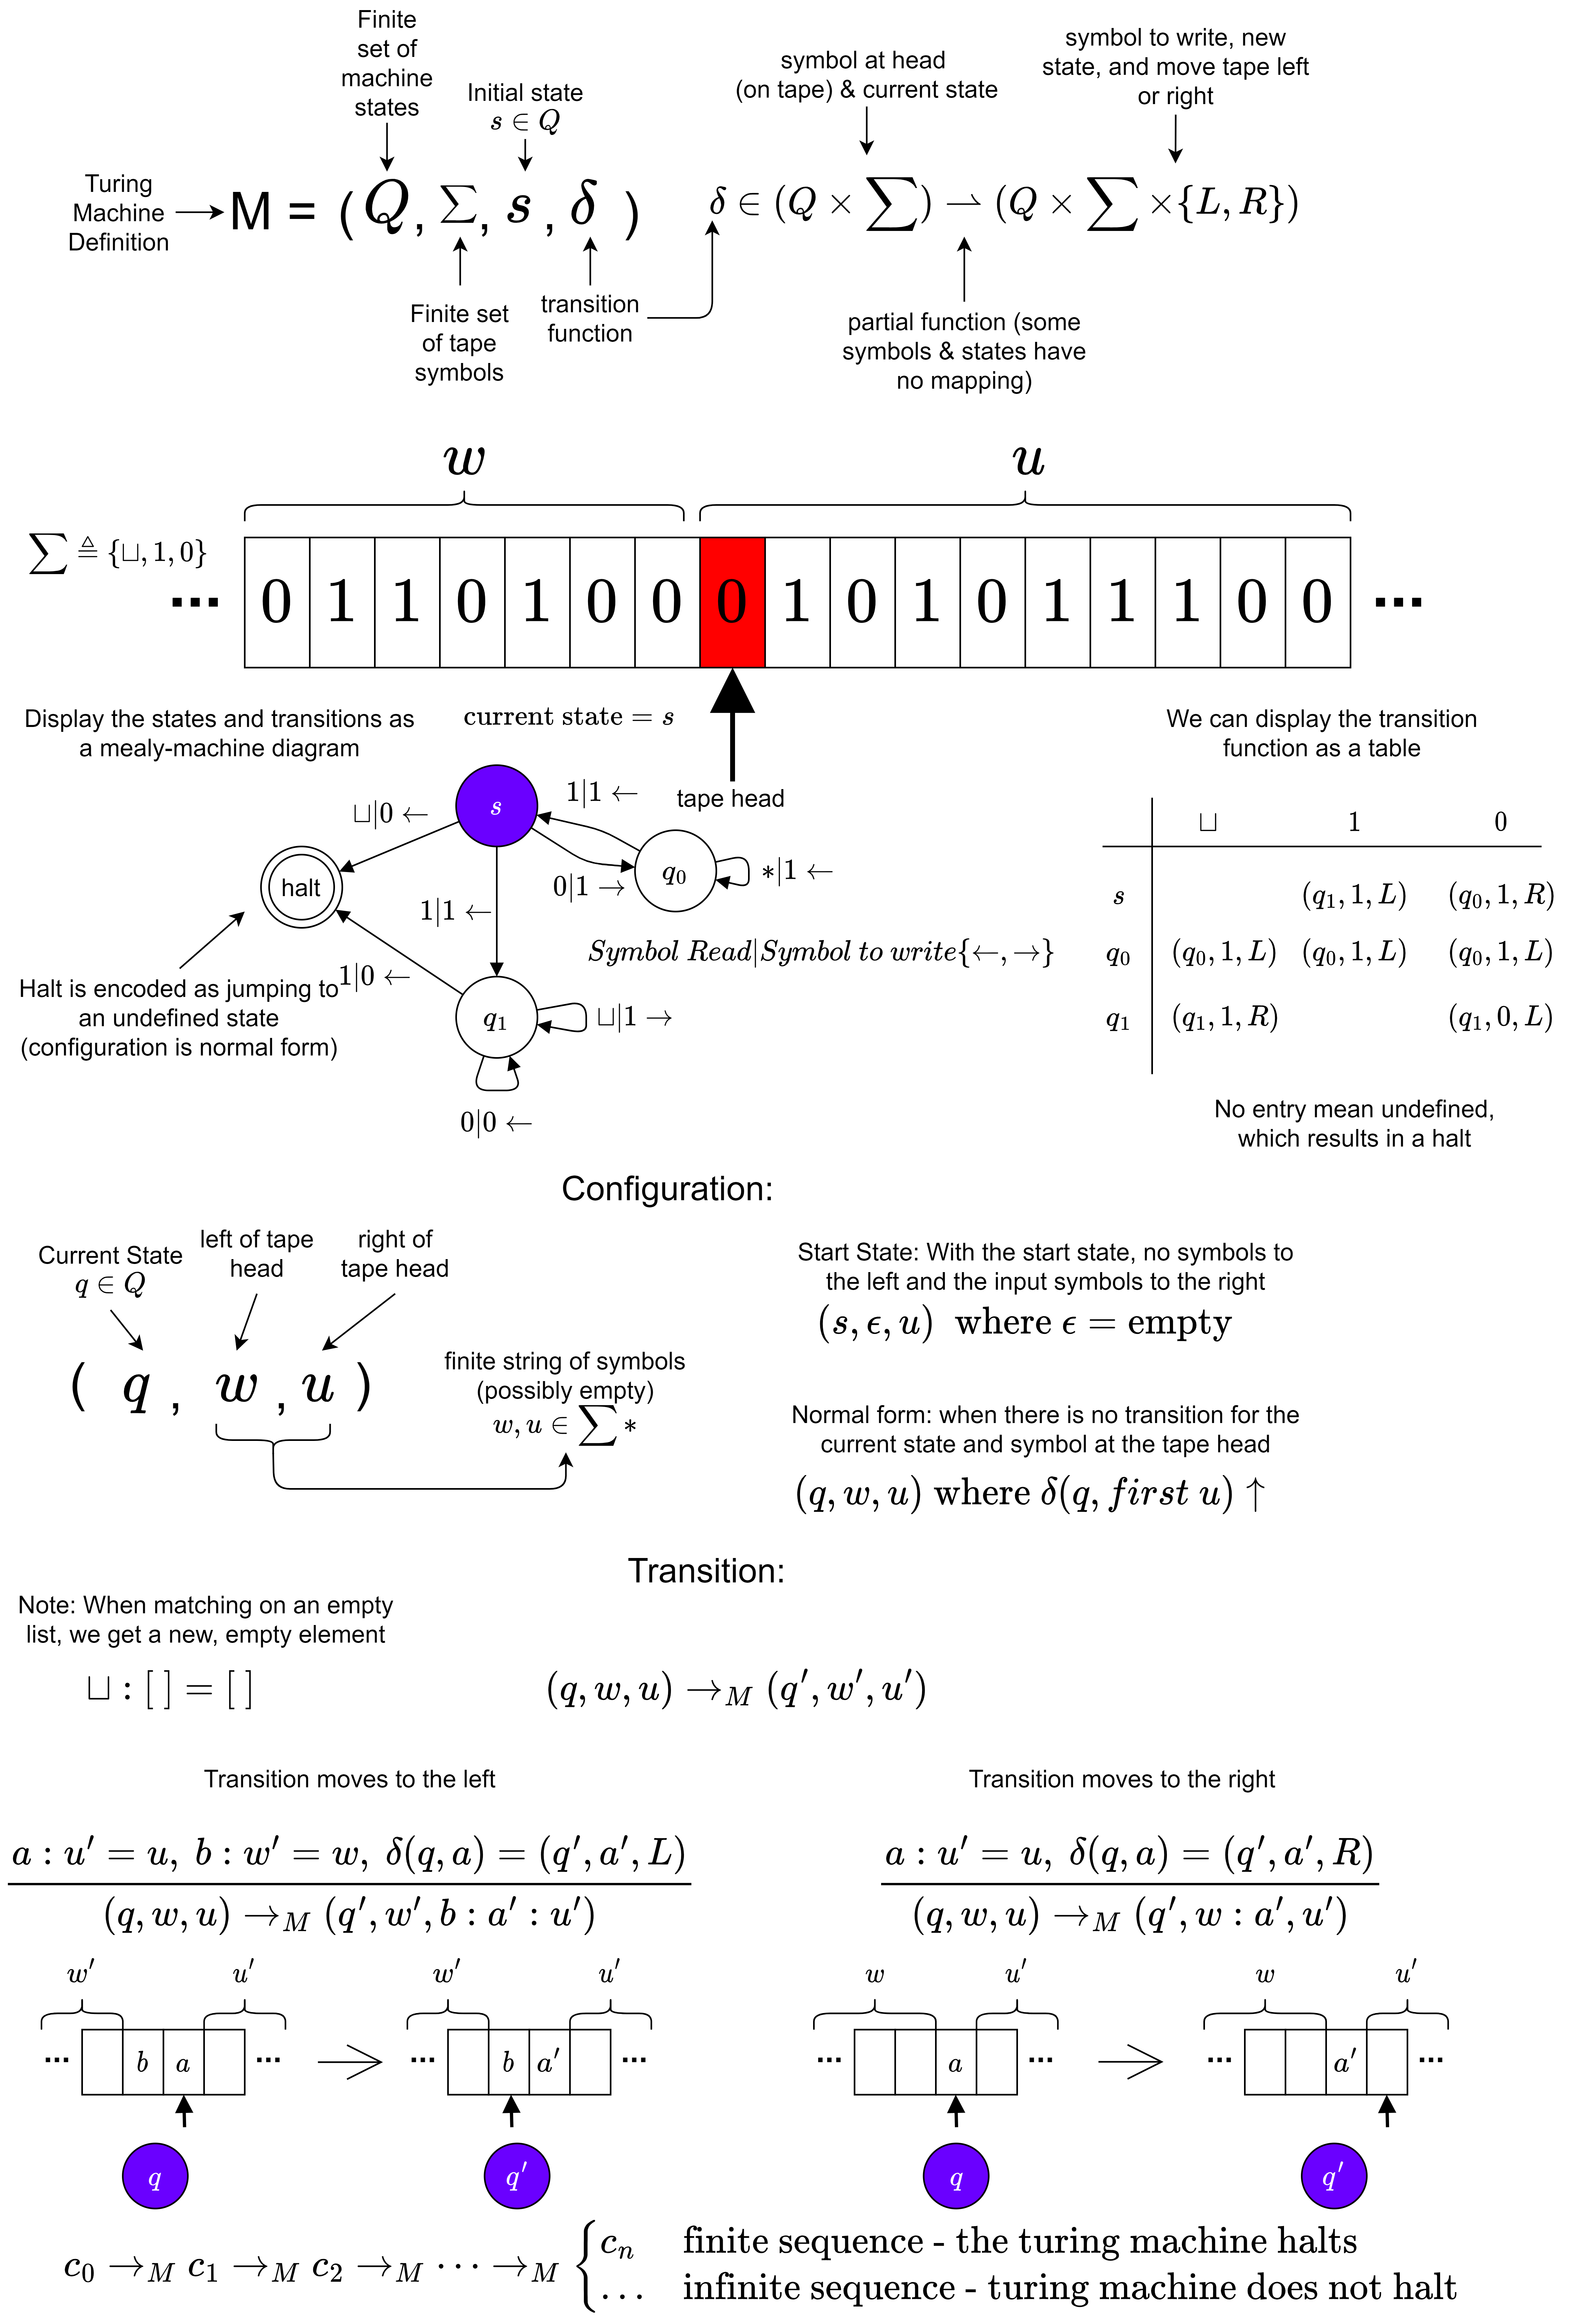
\includegraphics[width=0.7\textwidth]{turing_machines/images/turing_machine.drawio.png}
    \end{center}
\end{definitionbox}

\textit{Register machines} abstract away the representation of numbers and operations on numbers (just uses $\mathbb{N}$ with increment, decrement operations), \textit{Turing machines} are a more concrete representation of computing.

\subsection{Turing $\to$ Register Machine}
We can show that any computation by a \textit{Turing Machine} can be implemented by a \textit{Register Machine}. Given a \textit{Turing Machine} $M$:
\begin{enumerate}
	\item Create a numerical encoding of $M$'s finite number of states, tape symbols, and initial tape contents.
	\item Implement the transition table as a register machine.
	\item Implement a register machine program to repeatedly carry out $\to_M$
\end{enumerate}
Hence \textit{Turing Machine Computable} $\Rightarrow$ \textit{Register Machine Computable}.

\subsubsection{Turing Machine Number Lists}
In order to take arguments, and return value we need to encode lists on number on the tape of a turing machine. This is done as strings of unary values.
\begin{center}
    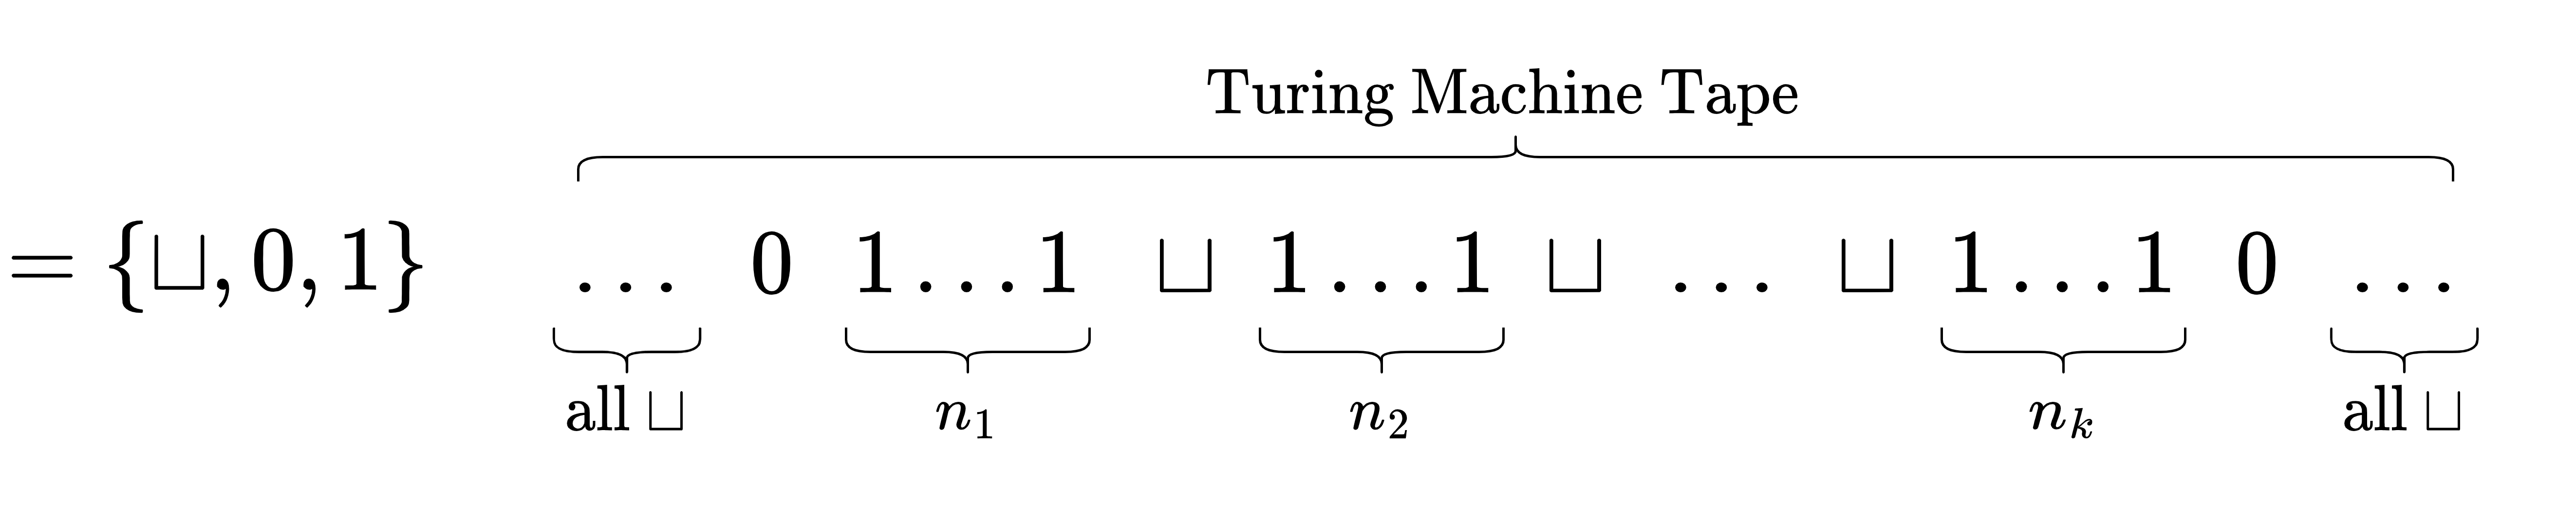
\includegraphics[width=0.8\textwidth]{turing_machines/images/turing_tape_list.drawio.png}
\end{center}
\begin{definitionbox}{Turing Computable}
	If $f: \mathbb{N}^n  \rightharpoonup \mathbb{N}$ is \textit{Turing Computable} iff there is a turing machine $M$ such that:
	\\
	\\ From initial state $(s, \epsilon, [x_1, \dots, x_n])$ (tape head at the leftmost $0$), $M$ halts if and only if $f(x_1, \dots, x_n)\downarrow$, and halts with the tape containing a list, the first element of which is $y$ such that $f(x_1, \dots, x_n) = y$.
	\\
	\\ More formally, given $M = (Q, \sum, s, \delta)$ to compute $f$:
	\[f(x_1, \dots, x_n)\downarrow \land f(x_1, \dots, x_n)=y \Leftrightarrow(s,\epsilon, [x_1, \dots, x_n]) \to^*_M (*, \epsilon, [y, \dots])\]
\end{definitionbox}

\subsubsection{Register $\to$ Turing Machine}
It is also possible to simulate any register machine on a turing machine. As we can encode lists of numbers on the tape, we can simply implement the register machine operations as operations on integers on the tape.
\\
\\ Hence \textit{Register Machine Computable} $\Rightarrow$ \textit{Turing Machine Computable}.

\subsubsection{Notions of Computability}
Every computable algorithm can be expressed as a turing machine (\textit{Church-Turing Thesis}). In fact \textit{Turing Machines}, \textit{Register Machines} and the \textit{Lambda Calculus} are all equivalent (all determine what is computable).

\begin{itemize}
	\item \textbf{Partial Recursive Functions} Godel and Kleene (1936)
	\item \textbf{$\lambda$-Calculus} Church (1936)
	\item \textbf{canonical systems for generating the theorems of a formal system} Post (1943) and Markov (1951)
	\item \textbf{Register Machines} Lambek and Minsky (1961)
	\item \textbf{And many more \dots} (multi-tape turing machines, parallel computation, turing machines embeded in cellular automata etc)
\end{itemize}